\chapter*{付録} %chapter 7 Appendixのように表示させない
\renewcommand{\thechapter}{S} %章番号をAに設定
\addcontentsline{toc}{chapter}{付録} %tocには表示
\setcounter{equation}{0} %式番号をリセット
\setcounter{figure}{0} %図番号をリセット

\begin{figure}[!ht]
  \begin{center}
    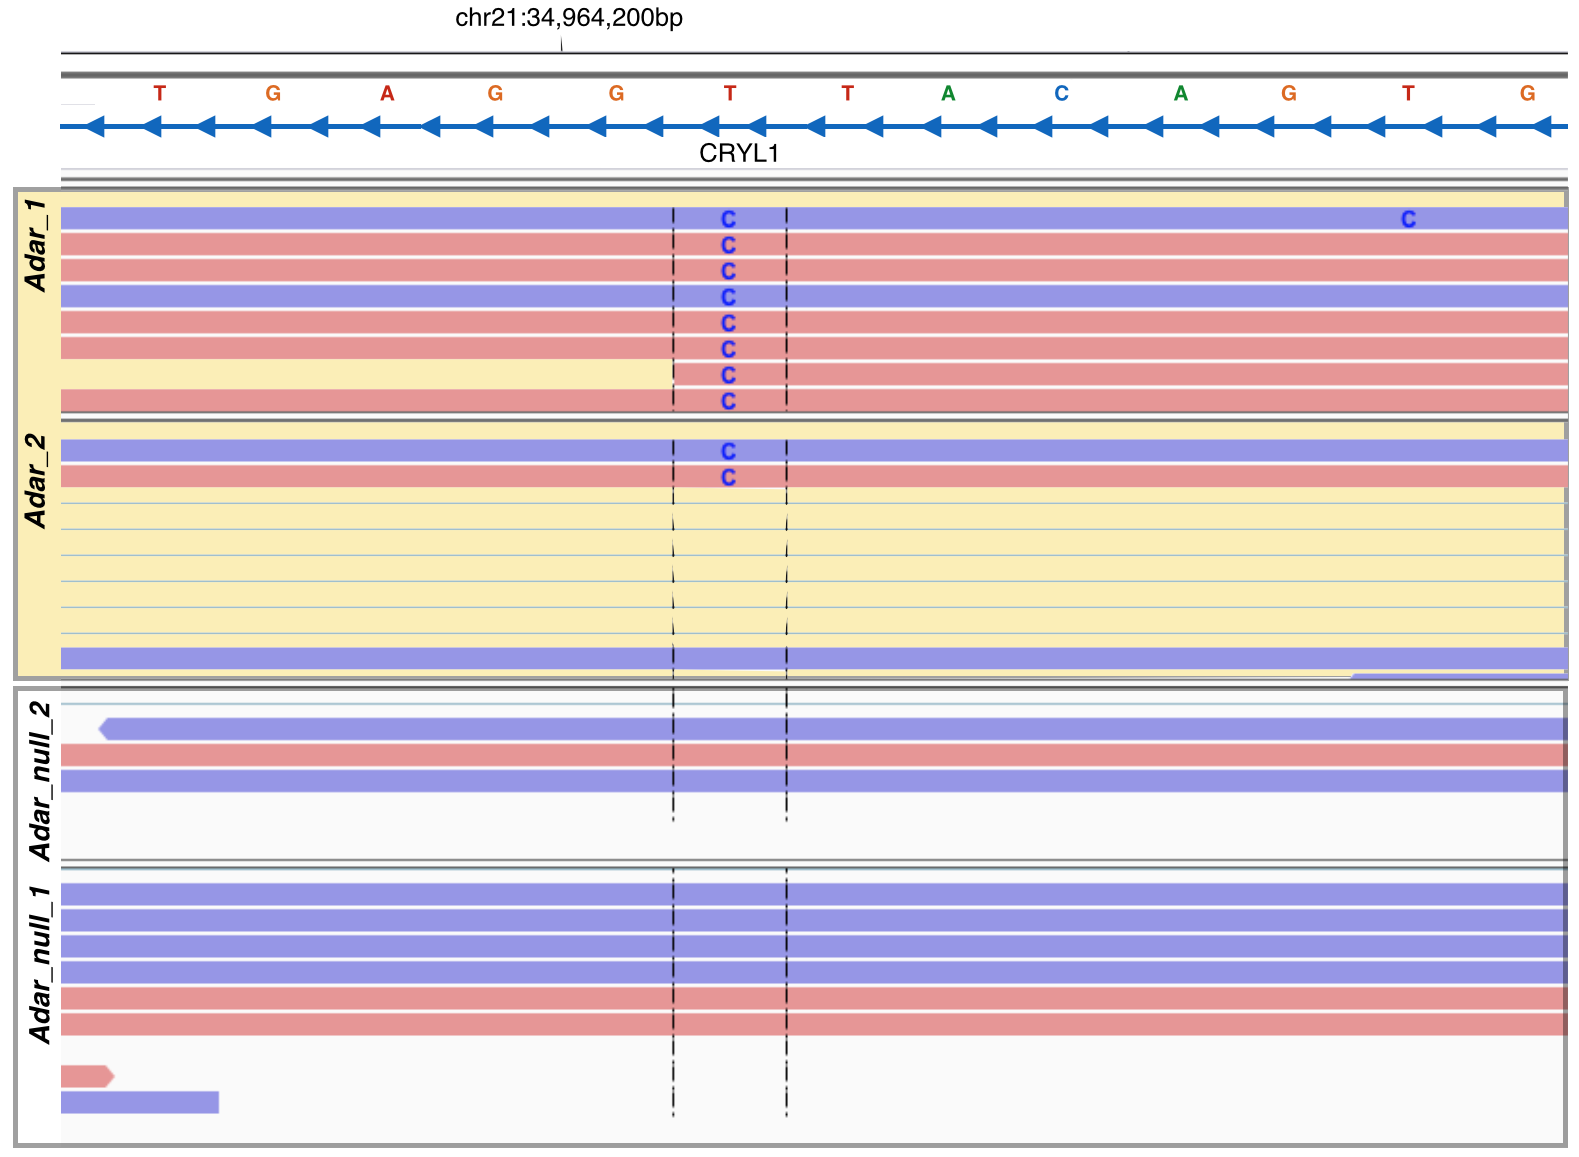
\includegraphics[width=0.8 \hsize]{Adar_eg.png}
  \end{center}
  \caption{アンチセンス鎖におけるA-to-I編集サイト}
  \begin{flushleft}
    \small{ivyによって検出されたA-to-I編集サイトを可視化した結果を示す。黄色くハイライトされたトラックは、\textit{Adar}が発現しているサンプルを示し、白いトラックはsiRNAによるノックダウン株の結果である。このCRYL1遺伝子はアンチセンス鎖から発現しているため、A-to-I編集サイトは、その逆鎖であるT-to-Cミスマッチとして検出される。転写物の方向性を考慮しない場合、こういったサイトはA-to-I編集サイトとして検出することは難しい。}
  \end{flushleft}
  \label{fig:visual}
\end{figure}

